\documentclass[10pt,twocolumn]{article}
\usepackage[margin=.73in]{geometry}
\usepackage[T1]{fontenc}\usepackage{lmodern,microtype,booktabs,amsmath,graphicx,float,natbib,hyperref,balance}
\newcommand{\Description}[1]{}
\renewcommand{\thefigure}{S\arabic{figure}}\renewcommand{\thetable}{S\arabic{table}}
\newcommand{\PrimaryRows}{%
Qwen3.6 & Base & 0.13132 & 0.13008 & $+0.00123$ $[-0.00053,+0.00363]$ & .022\\
Qwen3.6 & Wrong persona & 0.13132 & 0.17410 & $-0.04278$ $[-0.04781,-0.03696]$ & .022\\
Qwen3.6 & OPRO & 0.13132 & 0.13152 & $-0.00020$ $[-0.00143,+0.00083]$ & 1.000\\
Qwen3.6 & Ridge & 0.13132 & 0.10955 & $+0.02177$ $[+0.01974,+0.02417]$ & .022\\
Granite & Base & 0.13594 & 0.13656 & $-0.00063$ $[-0.00199,+0.00098]$ & .023\\
Granite & Wrong persona & 0.13594 & 0.16819 & $-0.03225$ $[-0.03572,-0.02824]$ & .022\\
Granite & Native GigaEvo & 0.13594 & 0.13670 & $-0.00076$ $[-0.00400,+0.00385]$ & .022\\
Granite & Ridge & 0.13594 & 0.10955 & $+0.02639$ $[+0.02455,+0.02834]$ & .022\\%
}

\newcommand{\AllRows}{%
GA & $+0.00118$ $[+0.00053,+0.00178]$ & .022 & $-0.00136$ $[-0.00206,-0.00074]$$^{\dagger}$ & .022\\
DE & $+0.00089$ $[-0.00007,+0.00201]$ & .022 & $-0.00116$ $[-0.00249,+0.00058]$ & .022\\
PromptBreeder & $+0.00246$ $[-0.00069,+0.00495]$ & .022 & $-0.00053$ $[-0.00235,+0.00251]$ & .023\\
MAP-Elites-style & $+0.00123$ $[-0.00053,+0.00363]$ & .022 & $-0.00063$ $[-0.00199,+0.00098]$ & .023\\
GEPA-style & $+0.00010$ $[-0.00151,+0.00145]$ & 1.000 & $-0.00087$ $[-0.00322,+0.00170]$ & .022\\
Official GEPA & $-0.00020$ $[-0.00122,+0.00101]$ & 1.000 & $-0.00045$ $[-0.00168,+0.00061]$ & .842\\
Native GigaEvo & $-0.00009$ $[-0.00130,+0.00104]$ & 1.000 & $+0.00014$ $[-0.00280,+0.00213]$ & 1.000\\
OPRO & $+0.00143$ $[-3.2\times10^{-6},+0.00308]$ & .022 & $+0.00074$ $[-0.00136,+0.00420]$ & .022\\
ProTeGi & $+0.00244$ $[+0.00101,+0.00405]$ & .022 & $-0.00250$ $[-0.00343,-0.00174]$$^{\dagger}$ & .022\\
Random & $+0.00086$ $[+0.00039,+0.00133]$ & .022 & $+0.00115$ $[-0.00128,+0.00444]$ & .022\\
Best-of-budget & $-0.00044$ $[-0.00112,+0.00020]$ & .272 & $-0.00171$ $[-0.00211,-0.00131]$$^{\dagger}$ & .022\\
\midrule
GA, calibrated fitness & $-0.00044$ $[-0.00104,+0.00016]$ & .582 & $-0.00266$ $[-0.00318,-0.00213]$$^{\dagger}$ & .022\\
GA, legacy fitness & $+0.00080$ $[+3.0\times10^{-7},+0.00164]$ & .022 & $-0.00166$ $[-0.00255,-0.00082]$$^{\dagger}$ & .022\\
MAP-Elites, calibrated fitness & $-0.00034$ $[-0.00099,+0.00030]$ & 1.000 & $-0.00267$ $[-0.00377,-0.00179]$$^{\dagger}$ & .022\\%
}

\newcommand{\SeedRows}{%
Qwen3.6 & GA, raw & 0.15665 & 0.13127 & +0.00132, +0.00134, +0.00087\\
Qwen3.6 & GA, calibrated & 0.16377 & 0.12965 & -0.00066, +0.00003, -0.00069\\
Qwen3.6 & MAP-Elites, raw & 0.15577 & 0.13132 & -0.00053, +0.00045, +0.00378\\
Qwen3.6 & MAP-Elites, calibrated & 0.17042 & 0.12976 & -0.00029, -0.00087, +0.00015\\
Granite & GA, raw & 0.17209 & 0.13520 & -0.00090, -0.00195, -0.00123\\
Granite & GA, calibrated & 0.18219 & 0.13391 & -0.00295, -0.00280, -0.00223\\
Granite & MAP-Elites, raw & 0.17640 & 0.13594 & -0.00202, -0.00096, +0.00110\\
Granite & MAP-Elites, calibrated & 0.18436 & 0.13389 & -0.00203, -0.00385, -0.00214\\%
}

\title{Supplement S4: Historical diagnostics}\author{Anonymous authors}\date{}\begin{document}\maketitle
\section{Source-data identity audit}
A separate CPU audit compared the derived corpus with the original
\href{https://osf.io/q9jrh}{IPIP120.dat} from Johnson's data repository.
The article describes the IPIP-NEO-120 study~\cite{johnson2014ipip}; the
later OSF deposit linked here supplies the audited source file.
The original file contains 619,150 records. All 410,168 retained derived
records matched exactly by case identifier and the 120 recoded item values:
zero absent cases and zero item mismatches. The source file's SHA-256 was
checked against its published OSF metadata, and the derived corpus's SHA-256
matched the frozen experiment input before and after the audit. Only aggregate
counts were exported; respondent records used private temporary storage.
The original DAT120 codebook confirms that reverse-keyed items were already
recoded and zero denotes missingness. No second reversal was applied.
This verifies retained case/item identity, not demographic-field equivalence,
completeness of the historical filtering procedure, participant consent,
upstream data permissions, or absence from pretraining. The audit did not
estimate predictive performance or inspect panel-specific outcomes.

\section{Scope}
The evidence map in Table~\ref{tab:evidence-map} distinguishes the analysis families.
These additional analyses are post hoc, using the exposed original 600-person
cohort and three search seeds. They do not supply a new confirmatory sample.
Original 110-test results are unchanged. The initial representation tests use one
33-test Holm family; direct objective and interaction tests use a separate
nine-test family. The figure/table differences are computed from unrounded
values. Intervals for LLM comparisons cross respondents and observed search
seeds; sign-flip p-values condition on those seeds. Ridge-only contrasts
resample respondents with trained predictors held fixed.

\begin{table*}[t]\centering\small
\caption{Raw and calibrated losses of the same selected templates; the final
column lists three seed-specific calibrated differences from each cell's base.}
\begin{tabular}{@{}llrrl@{}}\toprule
Model & Search family, fitness & Raw RPS & Calibrated RPS & Differences by seed\\\midrule
\SeedRows
\bottomrule\end{tabular}\end{table*}

\paragraph{Objective contrasts.}
The first four contrasts are raw-fitness minus calibrated-fitness RPS.
Positive values favor calibrated fitness. Remaining rows subtract these
paired objective effects; they are not inferred from subgroup significance.
All five interaction intervals contain zero. No effect is claimed to generalize
to an unseen optimizer seed. The smallest possible two-sided sign-test p-value
with three seed pairs is .25; the table instead uses respondent-level sign flips
after averaging the three seeds.
\begin{table*}[t]\centering\small
\caption{All nine post-hoc objective contrasts. Intervals cross respondents and observed seeds; Holm $p$ values condition on the three frozen runs.}
\begin{tabular}{@{}lrrr@{}}\toprule
Contrast & Difference & Crossed 95\% interval & Conditional $p_{\rm H}$\\\midrule
Qwen:GA:raw--calibrated & +0.00163 & [+0.00111,+0.00219] & 0.002\\
Qwen:MAP:raw--calibrated & +0.00156 & [-0.00012,+0.00347] & 0.002\\
Granite:GA:raw--calibrated & +0.00130 & [+0.00060,+0.00204] & 0.002\\
Granite:MAP:raw--calibrated & +0.00205 & [+0.00015,+0.00340] & 0.002\\
Qwen: GA--MAP objective & +0.00007 & [-0.00190,+0.00206] & 0.719\\
Granite: GA--MAP objective & -0.00075 & [-0.00249,+0.00185] & 0.002\\
GA:Qwen--Granite & +0.00033 & [-0.00028,+0.00099] & 0.252\\
MAP:Qwen--Granite & -0.00049 & [-0.00158,+0.00049] & 0.047\\
Optimizer--model interaction & +0.00082 & [-0.00029,+0.00211] & 0.012\\
\bottomrule\end{tabular}\end{table*}

\section{Representation controls}
Categorical ridge uses 175 one-hot features: five categories for each of
30 facets and five traits. Continuous ridge uses the same 35 values before
discretization, standardized on training people. Both use 8,000 training and
120 selection respondents, choosing penalty from $\{1,10,100,1000\}$ before
reading evaluation labels. Selected penalties are 100 and 1, respectively.
Categorical, continuous and raw-history ridge score 0.11384, 0.11558 and
0.10955. Their pairwise differences (categorical--raw, continuous--raw,
categorical--continuous) are 0.00428, 0.00603 and $-0.00174$; corresponding
95\% intervals are $[.00378,.00478]$, $[.00540,.00664]$ and
$[-.00231,-.00120]$. All have Holm $p=.006599$. These are fitted-model
gaps, not a causal decomposition or an information bound.

\section{Search ranking diagnostic}
Each observed pool contributes the first complete evaluation per distinct
candidate. We compare the saved raw and cross-fitted-calibrated scores,
excluding tied pairs from the discordance denominator. The 24 pools span both
models, three seeds, two optimizers and two objectives. Median Spearman
correlation is .344, median discordant fraction .356, and median overlap of the
two top-five sets is zero. These are within-search descriptors, not independent
hypothesis tests or evidence of causal mediation.

\paragraph{Independent summary recomputation.}
A separate implementation reconstructed the 48 mixture-screen and 24
prior-anchored extension comparisons from the retained individual loss arrays.
For all 72 contrasts it exactly reproduced the mean differences, 5,000-draw
respondent-bootstrap intervals, conditional sign-flip probabilities, Holm
adjustments and joint screen decisions. The same declared random stream was
used for numerical comparison. This check validates aggregation from saved
losses; it does not regenerate model forecasts, refit predictors, or provide
independent confirmation of the adaptive scientific findings. The aggregate
receipt and checking source accompany the evidence bundle; individual losses
remain on the research host.

\section{Artifact inventory}
Machine-readable aggregates contain all 33 representation contrasts and all 9
objective contrasts, plus 24 history summaries. The fixed diagnostic protocol,
analysis scripts and figure scripts accompany this local draft. Raw human
records remain on the research host. Their inclusion in an anonymous release
requires a separate permission and de-identification review; this local
inventory is not a claim that a public release already exists.
\begin{table*}[t]\centering\small
\caption{Distinct analysis families. Original post-hoc families reuse the
exposed Evaluate600; fixed-template transfer uses 600 additional people from
the same corpus. Holm corrections are within families, not across the adaptive
research program.}\label{tab:evidence-map}
\begin{tabular}{@{}p{.25\textwidth}p{.23\textwidth}p{.40\textwidth}@{}}\toprule
Question / family & Status & Target and interpretation\\\midrule
Primary and original arm contrasts / 110 & Frozen before evaluation & Respondent mean over three frozen runs; crossed intervals also resample observed runs.\\
Representation / 33 & Post hoc & Fitted-model comparison at 8,000 labels, same exposed people.\\
Objectives and interactions / 9 & Post hoc & Direct run-index paired effects, conditional sign flips; three seeds.\\
Ordinary budget / 48; shared-prior budget / 48 & Sequential adaptive diagnostics & Fixed fitted predictors at each budget, three LLM runs; separate families.\\
Mixture screen / 48 & Adaptive exploratory & Respondent effects conditional on nine fixed fit/run combinations; no optimizer or subset resampling.\\
Anchored rival / 24 & Subsequent adaptive extension & Frozen original hybrid versus prior-anchored ridge and its neutral mixture; same nine fixed combinations.\\
Readout replay / 4 intervals & Engineering diagnostic & Calibration-only numerical compatibility, separate from predictive improvement.\\
Selected-template replay / 4 primary + 4 secondary & Frozen replay on exposed data & Two fresh-server rounds of the GA objective contrast; separate Holm-four families. No new optimizer runs or people.\\
Additional-respondent transfer / 3 primary & Fixed after original outcomes & Historical GA/MAP winners on 600 inventoried-disjoint same-corpus people; three Granite tests, conditional on old seeds. Qwen and ridge are mandatory diagnostics.\\
Same-shortlist selector / 10 & Subsequent exploratory intervention & Five candidates from each of 12 archived GA pools; raw versus cross-fitted calibrated selection, then the old exposed Evaluate600. Four selector effects, four search effects, two interactions; three old seeds.\\\bottomrule
\end{tabular}\end{table*}


\clearpage\onecolumn
\section{Full method visualization}
\begin{center}
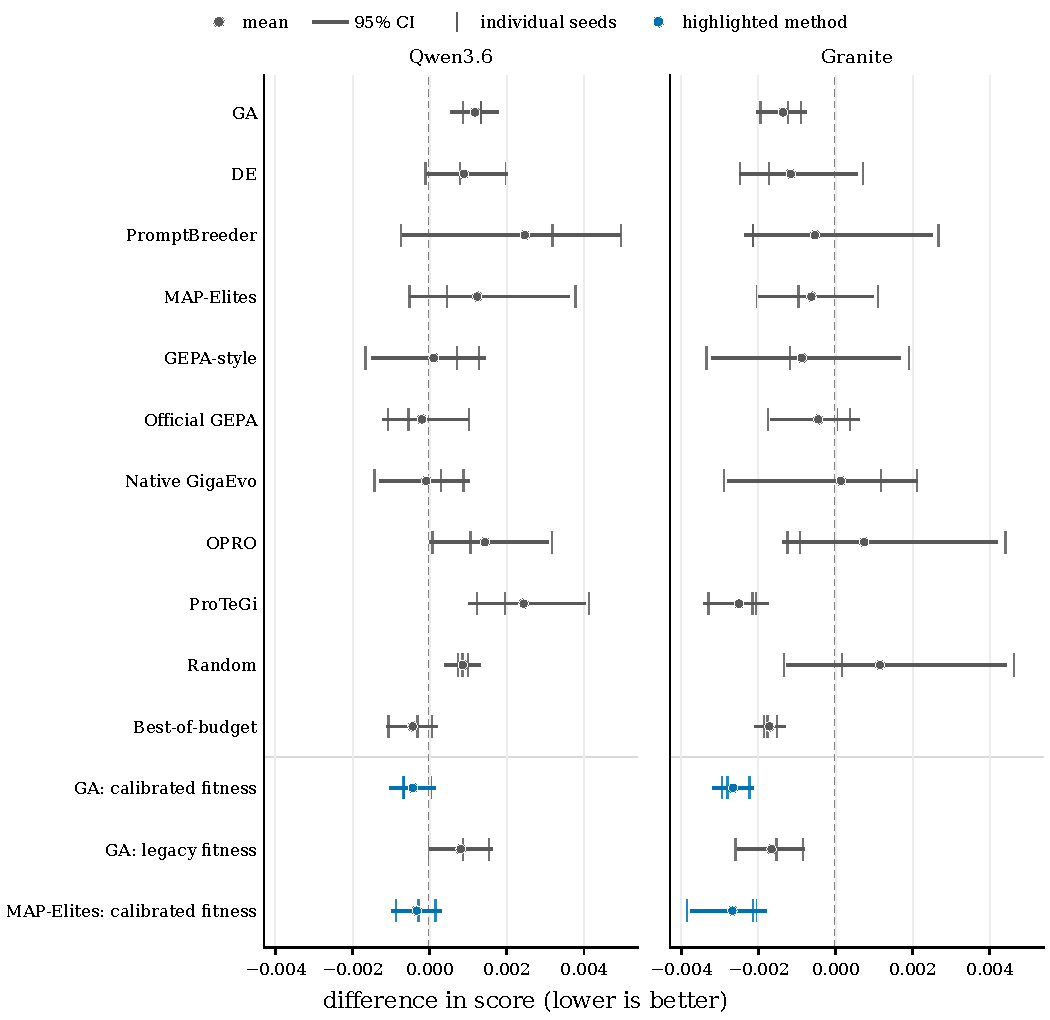
\includegraphics[width=.90\textwidth]{assets/99a7b3e5d11c.pdf}
\end{center}
\noindent\textbf{Figure S1.} All 14 method/objective identities relative to their
own base. Circles are mean differences, bars are crossed 95\% intervals,
and ticks are seed values. Blue highlights calibrated-fitness variants.
The family remains the original 110 comparisons.
\clearpage
\section{Paired MAP-Elites objective effects}
\begin{center}
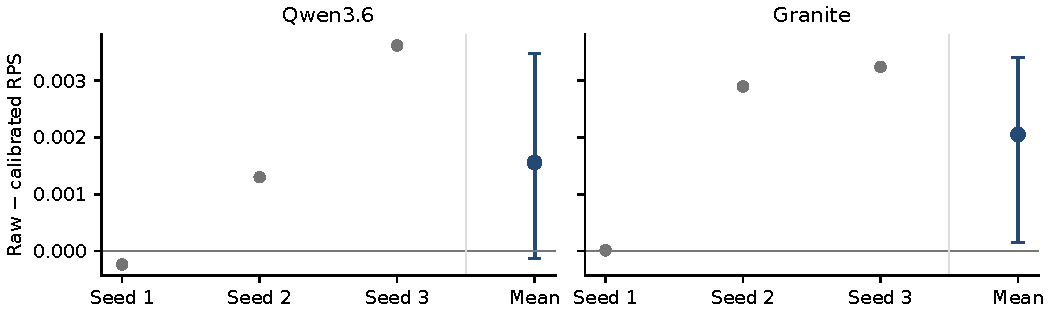
\includegraphics[width=.98\textwidth]{assets/5220d2537bbe.pdf}
\end{center}
\noindent\textbf{Figure S2.} All paired MAP-Elites seed effects and overall
crossed interval. Seeds are paired by initialization index, not a shared
mutator-sample trajectory. Points show independent search runs. Positive favors calibrated fitness.

\section{Calibration-only readout repeatability}
An engineering replay used the same neutral persona, pinned source and serving
configuration, and all 120 calibration people twice per model. No search or
new evaluation-person forecast was run. A pointwise probability tolerance of
$5\times10^{-4}$ failed; archived original runs also fail that tolerance against
their shared reference. Before reading the new full-panel replay results, a
dated amendment fixed a separate calibration-score compatibility criterion:
four paired respondent-bootstrap 98.75\% intervals, each wholly within
$[-0.0001,+0.0001]$ RPS (20,000 draws; Bonferroni-four interval levels).
The margin is below 8\% of the smaller exploratory GA objective effect.
This is a post-failure engineering amendment, not an original scientific
preregistration or a claim of population equivalence.

Source, model, configuration, current token reconstruction, repeated token
sequences, person/item order, probabilities and costs passed their checks.
Three raw-RPS comparisons passed the amended interval rule. Qwen repeat 2
had mean difference $+0.0000700$ and interval $[-0.0001570,+0.0002709]$,
which failed. All four comparisons and failed pointwise probes were retained;
the planned new-seed search was not released. The observed score variation
does not establish its cause, invalidate every original effect estimate, or
bound optimized-candidate variability. Historical token sequences were not
saved, so present reconstruction cannot retrospectively prove their identity.

\begin{table}[H]\centering\small
\caption{Calibration replay versus historical neutral readout. Intervals are
98.75\% paired respondent intervals; the fixed compatibility margin is
$\pm0.0001$. These differences are not optimized-template uncertainty bounds.}
\begin{tabular}{@{}lrrl@{}}\toprule
Replay & Mean raw RPS change & Interval & Within margin\\\midrule
Qwen 1 & +0.0000121 & [-0.0000012,+0.0000364] & Yes\\
Qwen 2 & +0.0000700 & [-0.0001570,+0.0002709] & No\\
Granite 1 & +0.0000011 & [0,+0.0000034] & Yes\\
Granite 2 & +0.0000001 & [-0.0000036,+0.0000030] & Yes\\\bottomrule
\end{tabular}\end{table}
For scale, the saved three-run GA raw-minus-calibrated effects are 0.00163
(Qwen) and 0.00130 (Granite); the planned Granite MAP-Elites effect is 0.00205.
The replay intervals concern neutral calibration forecasts, whereas these
scientific effects concern selected-template evaluation forecasts. The saved
forecast scores reproduce exactly; serving-level repeatability remains open.

\paragraph{Concurrency intervention.}
A subsequent frozen engineering protocol restarted the Qwen server for four
blocks with request concurrency $4,1,1,4$, each replaying the same 120-person
neutral calibration panel twice. All 57,600 forecasts completed with identical
prompt-token hashes. Within-server respondent RPS root-mean-square differences
were $0.000118$, $0.000979$, $0.001071$, and $0.000084$, respectively.
Serial requests therefore did not repair repeatability in this diagnostic.
Six of eight historical-reference intervals extended beyond the original
$\pm0.0001$ margin, including both replays of the final concurrency-four block
despite its small within-server difference. These intervals are descriptive
diagnostics, not a new multiplicity-controlled acceptance test. Two blocks per
setting do not identify a particular numerical kernel as the cause or bound
optimized-template variation. The additional-seed scientific campaign remains
blocked; no failed replay was replaced or tolerance relaxed.

\section{Selected-template serving robustness}
A separate protocol fixed two complete replay rounds before new inference.
Each round covers both models, both GA fitness objectives and all three
historical template seeds: 24 cells in total, each with a fresh server and
the unchanged final runner. Selected templates, model locks, input panels,
source hashes, the 8,000-person prior and historical results were preserved.
Each cell repeats base/evolved calibration on 120 people and
base/evolved/wrong-profile prediction on the same exposed 600 people.
There is no new search, prospective respondent sample or hybrid-mixture test.

The primary analysis refits calibration on the original calibration panel.
The secondary analysis transfers each historical calibration weight and CDF
center to the new evaluation forecasts. Each regime has four model-by-round
contrasts and a separate Holm-four correction. The frozen positive screen
requires all four positive differences, positive lower crossed-interval bounds
and adjusted $p<.05$. Intervals use 5,000 crossed respondent/template draws;
sign flips condition on the same three templates. Neither two serving rounds
nor resampling those templates estimates variation across new optimization runs.

\begin{table}[H]\centering\small
\caption{Complete frozen-template serving replay. Positive raw-minus-calibrated GA RPS favors calibrated fitness. Crossed 95\% intervals resample respondents and the three fixed templates; respondent sign-flip $p$ values are Holm-adjusted separately across four comparisons per calibration regime. These are two serving rounds on the same exposed people, not new optimizer runs.}
\label{tab:serving-replay}
\begin{tabular}{@{}llrrrr@{}}\toprule
Calibration & Model & Round & Difference & 95\% interval & Holm $p$\\\midrule
Refitted & Qwen & 1 & +0.00161 & [+0.00109,+0.00215] & 0.0008\\
Refitted & Qwen & 2 & +0.00159 & [+0.00108,+0.00212] & 0.0008\\
Refitted & Granite & 1 & +0.00130 & [+0.00059,+0.00203] & 0.0008\\
Refitted & Granite & 2 & +0.00130 & [+0.00059,+0.00203] & 0.0008\\
Fixed & Qwen & 1 & +0.00162 & [+0.00109,+0.00215] & 0.0008\\
Fixed & Qwen & 2 & +0.00160 & [+0.00109,+0.00213] & 0.0008\\
Fixed & Granite & 1 & +0.00130 & [+0.00059,+0.00203] & 0.0008\\
Fixed & Granite & 2 & +0.00130 & [+0.00059,+0.00203] & 0.0008\\
\bottomrule\end{tabular}\end{table}


Both regimes satisfy their four-contrast screen. All 12 seed-specific primary
differences are positive; the complete seed values and cell-level controls
are retained in the aggregate report. Calibration weights do not change in
any of the 48 base/evolved comparisons with historical values, although CDF
centers and probabilities can change. Across the 24 base/evolved evaluations
per model, mean refitted-RPS changes versus history range from
$-0.0000493$ to $+0.0000783$ for Qwen and $-0.00000281$ to $+0.00000109$
for Granite. Corresponding raw-RPS changes range from $-0.0000851$ to
$+0.0001075$ and from $-0.00000352$ to $+0.00000581$, respectively.
The largest individual probability-coordinate drift is 0.4337 for Qwen and
0.0617 for Granite; preserved aggregate contrasts therefore do not establish
pointwise reproduction. Wrong-profile minus evolved RPS remains positive in
every cell (Qwen 0.04078--0.04810; Granite 0.03164--0.03782).
Ridge fits and their saved losses are unchanged by this experiment.

All 24 cells complete with 2,937,600 confirmed forecasts, zero failed or
uncertain forecasts, and 3,596,132,160 reported prompt tokens. Slurm records
29,223 allocated single-GPU seconds (8.1175 GPU-hours), including server startup.
This is replay cost, not an end-to-end optimization-efficiency estimate.
All four primary contrasts were additionally recomputed from saved individual
losses by an independent statistics implementation; its receipt reports the
numerical agreement. The historical failed engineering gates remain failed.
These results support the observed GA contrast under the two tested serving
replays, not a repaired serving configuration or independent confirmation on
new people, optimizer trajectories, or behavioral outcomes.

\section{Additional-respondent fixed-template transfer}\label{sec:transfer}
After the original outcomes were inspected, a separate internal protocol
froze 24 historical selected GA/MAP-Elites-style templates: both models, two
search fitness objectives and three old seeds. The new 600 complete-case
respondents were sampled from 36,119 eligible people after exclusion of the
reachable inventoried historical exposure union. They come from the same
public IPIP120 corpus, so lifetime or model-pretraining exposure cannot be
excluded. Original Train8000 priors, Calibrate120 alpha and CDF centers,
frozen prompts, model snapshots and the selected same-history ridge
specification were reused. No new search or shortlist selection occurred;
this test does not evaluate the separate developmental aligned-selector
recipe. The internal freeze is not an external preregistration.

The three declared primary tests are Granite calibrated MAP versus raw MAP,
calibrated MAP versus its neutral base, and calibrated GA versus its neutral
base. Positive differences below are comparator minus calibrated-template
RPS. Crossed intervals resample respondents and the three \emph{observed}
search seeds; sign flips condition on those seeds. The original combined
decision rule requires a positive crossed interval and Holm $p<.05$ within
the three-test family. Qwen and other comparisons are diagnostics with their
uncorrected sign-flip $p$ values shown for completeness; their small values
are not additional declared primary successes.

\begin{table}[H]\centering\scriptsize
\caption{All eight E1 objective and neutral comparisons on the 600 additional
respondents. Positive favors the calibrated historical winner. Primary Holm
$p$ applies only to the three Granite tests marked P; the Granite MAP
calibrated-versus-raw interval crosses zero and fails the combined rule.}
\label{tab:e1-contrasts}
\begin{tabular}{@{}llllrr@{}}\toprule
Model & Arm & Contrast & $\Delta$ RPS [crossed 95\% CI] & Sign-flip $p$ & Primary $p_{\rm H}$\\\midrule
Qwen & GA & cal vs raw & $+0.001805$ [$+0.001358,+0.002257$] & .0002 & --\\
Qwen & GA & cal vs base & $+0.000337$ [$-0.000174,+0.000854$] & .1184 & --\\
Qwen & MAP & cal vs raw & $+0.001680$ [$+0.000007,+0.003393$] & .0002 & --\\
Qwen & MAP & cal vs base & $+0.000180$ [$-0.000506,+0.000806$] & .4043 & --\\
Granite & GA & cal vs raw & $+0.001229$ [$+0.000626,+0.001812$] & .0002 & --\\
Granite & GA & cal vs base (P) & $+0.002286$ [$+0.001661,+0.002893$] & .0002 & .0006\\
Granite & MAP & cal vs raw (P) & $+0.001523$ [$-0.000182,+0.002733$] & .0002 & .0006\\
Granite & MAP & cal vs base (P) & $+0.002156$ [$+0.001344,+0.003113$] & .0002 & .0006\\\bottomrule
\end{tabular}\end{table}

\begin{table}[H]\centering\scriptsize
\caption{Mandatory E1 controls for each calibrated historical winner. Values
are comparator minus calibrated-template RPS with crossed 95\% intervals;
negative ridge differences mean ridge is better. These diagnostics were not
in the three-test primary family.}
\label{tab:e1-controls}
\begin{tabular}{@{}lll l@{}}\toprule
Model & Arm & Same-history ridge minus template & Wrong-persona minus matched template\\\midrule
Qwen & GA & $-0.020850$ [$-0.021898,-0.019877$] & $+0.044778$ [$+0.041452,+0.048465$]\\
Qwen & MAP & $-0.020995$ [$-0.022161,-0.019898$] & $+0.041762$ [$+0.039263,+0.044285$]\\
Granite & GA & $-0.025188$ [$-0.026441,-0.023977$] & $+0.035653$ [$+0.032601,+0.038636$]\\
Granite & MAP & $-0.025318$ [$-0.026688,-0.023941$] & $+0.035213$ [$+0.031855,+0.038961$]\\\bottomrule
\end{tabular}\end{table}

All 24 cells have 600 people and 60 target items. The independent output gate
confirmed the original frozen lineage, 24 immutable attempts, serving logs,
probability and mass arrays, and $2{,}937{,}600$ requested and confirmed
forecasts with no failed or uncertain request. Prompt-token receipts sum to
$3{,}500{,}088{,}480$; these are new inference costs, not search costs.
The separately written finite CPU verifier reconstructed all 72 labelled
cell/control score rows, the selected ridge, all 16 contrast distributions
and the three-test Holm correction from saved raw forecasts and target labels;
its maximum discrepancy from the frozen analysis was
$8.33\times10^{-17}$. It shares the pinned CDF projection and ridge-fit
numerical primitives and does not independently regenerate model forecasts.

The same-history ridge, selected originally and refit on 8,000 old training
people with the same 60 observed answers, scores 0.10821 RPS here. Calibrated
GA/MAP means are 0.12906/0.12920 on Qwen and 0.13340/0.13353 on Granite.
The three observed Granite MAP seed effects against raw are
$-0.000288,+0.002381,+0.002477$; the first is unfavorable. A low answer-token
mass diagnostic for raw Granite MAP seed 3 is retained (mean 0.9473; 2.37\%
of target cells below 0.5), above the frozen mean-mass exclusion threshold.
Neither favorable base comparisons nor matched-versus-wrong-persona signals
establish optimizer superiority to ridge, new-search generalization, or
behavioral transfer.

\section{Exploratory same-shortlist selector intervention}
This E2 experiment reused the \emph{original exposed} Evaluate600, rather
than E1's additional 600 people. For each of the 12 archived GA trajectories
(two models, raw/calibrated search objectives, three seeds), the same five
historical candidates received new Select120 forecasts. Raw RPS and a fixed
two-fold cross-fitted calibrated RPS each selected one candidate from that
identical pool. Both choices were frozen before fresh Calibrate120/Evaluate600
inference, with a fresh neutral-base readback; one coincident pair was
deduplicated. There was no new search or new respondent cohort. The selection
stage confirmed 432,000 forecasts and the final stage 1,512,000, with zero
failed or uncertain requests; prompt-token receipts were 624,369,600 and
1,843,379,400, respectively. These are additional serving costs, not total
optimizer costs.

In Table~\ref{tab:e2-contrasts}, selector effects subtract raw-selector RPS
from calibrated-selector RPS within the named search objective. Search effects
subtract raw-search RPS from calibrated-search RPS within the named selector.
Negative values favor the first, calibrated option. The interaction is the
calibrated-selector search effect minus the raw-selector search effect.
Crossed 95\% intervals resample respondents and the three \emph{observed}
search seeds; respondent sign flips condition on those seeds, with Holm over
all ten two-sided tests. A favorable claim requires both a crossed interval
excluding zero and adjusted $p<.05$. The three seed columns are differences
on the fixed, paired archived trajectories, not new-search replicates.

\begin{table}[H]\centering\scriptsize\setlength{\tabcolsep}{3pt}
\caption{All ten E2 contrasts on the exposed original Evaluate600. Values are
calibrated RPS differences as defined in text; lower is better. All four
direct selector intervals include zero. The Qwen search effect under the raw
selector is the only interval wholly below zero; it is not selector benefit.}
\label{tab:e2-contrasts}
\begin{tabular}{@{}lp{.19\textwidth}lrrrc@{}}\toprule
Model & Contrast & $\Delta$ [crossed 95\% CI] & Seed 1 & Seed 2 & Seed 3 & $p_{\rm H}$\\\midrule
Qwen & Selector; calibrated search & $-0.000153$ [$-0.000495,+0.000181$] & $+0.000044$ & $-0.000434$ & $-0.000068$ & .3179\\
Qwen & Selector; raw search & $-0.000587$ [$-0.001456,+0.000044$] & $+0.000000$ & $-0.001541$ & $-0.000221$ & .0020\\
Qwen & Search; calibrated selector & $-0.000740$ [$-0.001712,+0.000308$] & $-0.001699$ & $+0.000376$ & $-0.000896$ & .0020\\
Qwen & Search; raw selector & $-0.001174$ [$-0.001852,-0.000562$] & $-0.001743$ & $-0.000730$ & $-0.001049$ & .0020\\
Qwen & Search $\times$ selector & $+0.000434$ [$-0.000152,+0.001131$] & $+0.000044$ & $+0.001107$ & $+0.000153$ & .0144\\\midrule
Granite & Selector; calibrated search & $-0.000013$ [$-0.000208,+0.000302$] & $+0.000249$ & $-0.000134$ & $-0.000154$ & .8352\\
Granite & Selector; raw search & $-0.000473$ [$-0.001334,+0.000104$] & $+0.000062$ & $-0.001435$ & $-0.000045$ & .0020\\
Granite & Search; calibrated selector & $-0.000171$ [$-0.001693,+0.001081$] & $-0.001782$ & $+0.001124$ & $+0.000143$ & .3179\\
Granite & Search; raw selector & $-0.000631$ [$-0.001872,+0.000357$] & $-0.001969$ & $-0.000177$ & $+0.000252$ & .0020\\
Granite & Search $\times$ selector & $+0.000460$ [$-0.000158,+0.001250$] & $+0.000187$ & $+0.001301$ & $-0.000109$ & .0020\\\bottomrule
\end{tabular}\end{table}

Calibrated selection changed 11 of 12 winners but none of its four direct
effects passes the combined interval-and-$p$ rule. The two raw-search
selector tests have small adjusted sign-flip probabilities despite crossed
intervals spanning zero; they are not declared improvements. Original
selection-audit attempt failed on a post-receipt server shutdown
diagnostic. Versioned selection gate classified that event explicitly
and passed the archived arrays; final gate and independent CPU readback
passed all 12 cells and ten contrasts. This operational chain does not
repair numerical serving compatibility. Compared with the historical base,
fresh Qwen base per-cell mean absolute RPS-loss drift was roughly
0.00031--0.00037 (maximum individual drift 0.0028--0.0048); Granite drift was
much smaller. All reported E2 contrasts therefore compare predictions within
the fresh serving execution. E2 does not test its selected winners on E1's
additional people, and E1 never evaluated those winners.

\section{Third-panel Granite-80 frozen-mixture transfer}\label{sec:hybrid-transfer}
This E3 test was designed after inspection of the original, E1, and E2
outcomes. Its internal protocol fixed the old Granite calibrated-GA n=80
recipe, controls, four contrasts, 0.001-RPS margin and inference before
opening the third panel's target answers; it is not an external
preregistration. The 600 complete-case respondents were sampled from 35,519
eligible cases after exclusion of 374,649 reachable inventoried case IDs,
including every original split and E1's additional Eval600. They are new to
these project panels, not a new sample recruited outside the public corpus;
unknown lifetime and model-pretraining exposure remain possible. The old
selected prompts, neutral prompts, Granite model snapshot, first-Cal60 scale
and CDF centers, old 60-person mixture-selection weights, penalties,
categorical/raw features, three disjoint 80-person ridge-fitting subsets,
and 8,000-person population prior were reused unchanged. Ridge penalties
were chosen on old Select120. The persona search consumed Search80 and
Select120 targets, and each new respondent supplies 60 observed answers;
``80-person'' names only the paired ridge-fit budget. The third-panel labels
selected none of these choices.

For each representation the optimized persona plus ordinary ridge was
compared with neutral persona plus prior-anchored ridge and neutral persona
plus the \emph{same} ordinary ridge. Each neutral arm retained its own old
selected mixture weight. The first control changes prompt, weight and ridge
centering; the second changes prompt and weight while holding ridge
coefficients fixed. Neither is an isolated prompt-only causal contrast.
The four planned comparator-minus-hybrid RPS gains form one two-sided Holm
family. Before paired respondent resampling, nine fixed per-person loss
vectors (three old search seeds by three fixed subset seeds) were
averaged, without ensembling forecasts or treating the nine combinations as
independent respondents. The fixed success rule requires each gain to be at
least 0.001, its paired respondent-bootstrap lower 95\% bound to exceed zero,
and its Holm-adjusted respondent sign-flip $p<.05$. Both controls must pass
for a representation; uncertainty conditions on those old choices.
The three n=80 subset seeds have pairwise overlap 0/0/0 and union 240 within
Train8000; the same sets are reused across representations and LLM seeds.
This index fact does not turn the nine fitted combinations into independent
respondent panels or new search replications.

\begin{table}[H]\centering\scriptsize
\caption{All four declared E3 contrasts on the third 600-person panel.
Positive gains favor the old optimized mixture; all pass the fixed gate.
The two-sided Holm family contains exactly these four rows.}
\label{tab:e3-full}
\begin{tabular}{@{}llrrr@{}}\toprule
Features & Neutral comparator & Gain & Paired 95\% CI & $p_{\rm H}$\\\midrule
Categorical & Prior-anchored & .001465 & [.001213,.001722] & .0008\\
Categorical & Same ordinary & .001843 & [.001595,.002088] & .0008\\
Raw & Prior-anchored & .001251 & [.001016,.001490] & .0008\\
Raw & Same ordinary & .001747 & [.001519,.001974] & .0008\\\bottomrule
\end{tabular}\end{table}

\begin{table}[H]\centering\scriptsize
\caption{E3 mean RPS component and mixture controls, lower is better.
Each row averages the nine fixed per-person loss vectors. The common full
8,000-person same-history ridge scores 0.10995, better than both hybrids.}
\label{tab:e3-components}
\begin{tabular}{@{}lrr@{}}\toprule
Predictor & Categorical & Raw\\\midrule
Optimized mixture & .132355 & .131532\\
Neutral + prior-anchored ridge & .133821 & .132784\\
Neutral + same ordinary ridge & .134198 & .133279\\
Optimized persona alone & .134180 & .134180\\
Neutral persona alone & .136691 & .136691\\
Prior-anchored ridge alone & .138871 & .137463\\
Ordinary 80-person ridge alone & .140831 & .139406\\
Full 8,000-person ridge & .109952 & .109952\\\bottomrule
\end{tabular}\end{table}

\begin{table}[H]\centering\scriptsize\setlength{\tabcolsep}{2.3pt}
\caption{Every E3 old-search-seed/subset combination. Subset indices 1--3
denote seeds 202610081--083. $w_O,w_N,w_A$ are the frozen optimized,
same-ordinary neutral and anchored-neutral persona weights; $H,N,A$ are
their respective third-panel mean RPS values. The nine rows per
representation are descriptive fixed combinations, not independent
replications.}
\label{tab:e3-combinations}
\resizebox{\columnwidth}{!}{%
\begin{tabular}{@{}lcrrrrrr@{}}\toprule
Features & Search/subset & $w_O$ & $w_N$ & $w_A$ & $H$ & $N$ & $A$\\\midrule
Categorical & 1/1 & .60 & .55 & .55 & .13229 & .13421 & .13373\\
Categorical & 1/2 & .65 & .60 & .50 & .13227 & .13415 & .13389\\
Categorical & 1/3 & .60 & .55 & .50 & .13228 & .13423 & .13384\\
Categorical & 2/1 & .65 & .55 & .55 & .13235 & .13421 & .13373\\
Categorical & 2/2 & .70 & .60 & .50 & .13236 & .13415 & .13389\\
Categorical & 2/3 & .65 & .55 & .50 & .13239 & .13423 & .13384\\
Categorical & 3/1 & .60 & .55 & .55 & .13239 & .13421 & .13373\\
Categorical & 3/2 & .65 & .60 & .50 & .13240 & .13415 & .13389\\
Categorical & 3/3 & .60 & .55 & .50 & .13246 & .13423 & .13384\\\midrule
Raw & 1/1 & .60 & .50 & .50 & .13158 & .13356 & .13295\\
Raw & 1/2 & .60 & .50 & .45 & .13137 & .13318 & .13275\\
Raw & 1/3 & .60 & .50 & .45 & .13125 & .13310 & .13265\\
Raw & 2/1 & .60 & .50 & .50 & .13178 & .13356 & .13295\\
Raw & 2/2 & .60 & .50 & .45 & .13156 & .13318 & .13275\\
Raw & 2/3 & .60 & .50 & .45 & .13146 & .13310 & .13265\\
Raw & 3/1 & .55 & .50 & .50 & .13179 & .13356 & .13295\\
Raw & 3/2 & .55 & .50 & .45 & .13154 & .13318 & .13275\\
Raw & 3/3 & .55 & .50 & .45 & .13146 & .13310 & .13265\\\bottomrule
\end{tabular}}
\end{table}

The frozen E3 preparation receipt has SHA256
\texttt{76f8a7b57f8b86793697824476105607}\allowbreak
\texttt{3930981c37d750a0b60b4673b9a6bf32};
the new panel's canonical hash is
\texttt{415583f53de73b7f0295f2c8a289cad1}\allowbreak
\texttt{bab311d9f0ce033a21ba840d6e1f8671}.
Preparation reproduced the old recipe and old-Eval losses before serving.
The independent output gate passed three immutable one-GPU attempts, each
with 72,000 requested/confirmed item forecasts and zero failed or uncertain
requests. The total was 216,000 forecasts and 237,089,520 reported prompt
tokens, excluding historical search, old calibration and CPU fitting cost.
The three allocated single-GPU elapsed times were 694, 622 and 640 seconds
(0.5433 GPU-hours total). Seed 3 recorded a post-receipt shutdown diagnostic;
its forecast arrays and counts passed the versioned gate, so this is not
silently removed. The independently written finite-CPU numerical verifier
recomputed all four gains, intervals, Holm values, component means and the
full-ridge control from archived raw forecasts and labels. Its maximum
absolute discrepancy was $9.38\times10^{-11}$, within the protocol's fixed
$10^{-10}$ tolerance. This readback did not regenerate model forecasts.
Neither this operational pass nor the favorable contrasts validate new
search trajectories, the E2 selector winners, Qwen serving compatibility,
external behavioral transfer, or superiority to the full ridge.

\section{Post hoc fixed-weight E3 readback}\label{sec:e4-fixed}
E4 reuses the already exposed E3 Eval600, frozen Granite prompts, saved
probabilities and n=80 ordinary ridge coefficients. Its question and analysis
were fixed internally only \emph{after} E3 effects had been inspected; no new
respondent panel or model inference was used. At the primary fixed weight
$w=.5$, each arm keeps its own historical first-Cal60 scale and CDF center,
but evolved and neutral forecasts share exactly the same ordinary ridge and
numeric weight. This removes unequal mixture weights from the comparison.
It identifies the effect of substituting an \emph{arm-specific calibrated
forecast package}, not prompt wording alone. The old last-Cal60
weight-selection labels are part of E3's lineage but their selected weights
are unused by this fixed-half primary comparison.

For each representation we average nine fixed \emph{per-person losses}
(three historical search seeds by three fixed ridge subsets) before pairing
the 600 respondents. The two neutral-minus-evolved fixed-half effects form a
separate, two-sided Holm family. The internally fixed descriptive gate
requires gain at least 0.001 RPS, positive paired respondent-bootstrap lower
95\% bound and adjusted respondent sign-flip $p<.05$. With 5,000 draws and
seed 20261021, both pass (Table~\ref{tab:e4-primary}). Intervals condition
on these old seeds/subsets and the exposed panel. The numerical verifier
recomputed every saved loss and statistic from the raw E3 forecasts with
maximum discrepancy zero; it shares the frozen CDF/RPS primitives and does
not regenerate model forecasts or create prospective confirmation.

\begin{table}[H]\centering\scriptsize
\caption{E4 fixed-half calibrated-package comparisons on exposed E3
respondents ($N=600$). Positive is neutral minus evolved RPS, lower scores
being better. Both rows form the Holm-2 family and pass the descriptive
0.001-RPS/positive-CI/adjusted-$p$ rule.}
\label{tab:e4-primary}
\resizebox{\columnwidth}{!}{%
\begin{tabular}{@{}lrrrr@{}}\toprule
Features & Evolved & Neutral & Gain [paired 95\% CI] & $p_{\rm H}$\\\midrule
Categorical & .132912 & .134389 & .001477 [.001291,.001676] & .0004\\
Raw & .131831 & .133279 & .001448 [.001264,.001643] & .0004\\\bottomrule
\end{tabular}}
\end{table}

\begin{table}[H]\centering\scriptsize
\caption{Complete \emph{fixed}, unselected E4 weight grid. Each entry is
the mean of nine fixed per-person loss vectors. Weight zero reproduces the
same ordinary ridge exactly for both arms. Other weights are descriptive;
no best weight was chosen from E3 labels.}
\label{tab:e4-grid}
\resizebox{\columnwidth}{!}{%
\begin{tabular}{@{}lrrrr@{}}\toprule
Features & $w$ & Evolved RPS & Neutral RPS & Neutral $-$ evolved\\\midrule
Categorical & 0 & .140831 & .140831 & .000000\\
Categorical & .25 & .135723 & .136517 & .000794\\
Categorical & .50 & .132912 & .134389 & .001477\\
Categorical & .75 & .132398 & .134447 & .002049\\
Categorical & 1 & .134180 & .136691 & .002512\\\midrule
Raw & 0 & .139406 & .139406 & .000000\\
Raw & .25 & .134378 & .135150 & .000772\\
Raw & .50 & .131831 & .133279 & .001448\\
Raw & .75 & .131765 & .133793 & .002028\\
Raw & 1 & .134180 & .136691 & .002512\\\bottomrule
\end{tabular}}
\end{table}

\begin{table}[H]\centering\scriptsize
\caption{Descriptive fixed-half sensitivity to the three \emph{old} Granite
search seeds. ``Leave out'' averages the remaining two seed means, each
already averaged across the three fixed n=80 ridge subsets. All values are
neutral-minus-evolved RPS; these are not new optimizer replications.}
\label{tab:e4-seeds}
\resizebox{\columnwidth}{!}{%
\begin{tabular}{@{}lrrrrrr@{}}\toprule
Features & Seed 1 & Seed 2 & Seed 3 & Leave out 1 & Leave out 2 & Leave out 3\\\midrule
Categorical & .001579 & .001317 & .001535 & .001426 & .001557 & .001448\\
Raw & .001546 & .001295 & .001504 & .001399 & .001525 & .001420\\\bottomrule
\end{tabular}}
\end{table}

At the same $w=.5$ but with raw \emph{uncalibrated} persona CDFs, the
descriptive neutral-minus-evolved gain is .005634 categorical (evolved
.141848, neutral .147482) and .005579 raw (evolved .140851, neutral .146430).
These gains are larger than the primary calibrated-package differences, yet
both arms' absolute RPS values are worse than their calibrated half-weight
counterparts. This secondary comparison has no additional claim threshold
or corrected-test status. It neither proves that calibration caused a
particular prompt effect nor isolates prompt text from other arm-specific
forecast differences.

The three E3 ridge subsets are reconstructed from the exact old
80-of-8,000 seeded permutations; pairwise intersections are 0/0/0 and their
union is 240 people. They sit \emph{inside} Train8000, are reused for both
representations and all three prompt seeds, and add no unique labelled people
beyond Train8000. Before evaluation, the original disjoint Train8000,
Search80, Select120 and Calibrate120 roles comprise 8,320 people and
499,200 target-item labels (8,320 $\times$ 60). Search80 supplied prompt
fitness, Select120 shortlist and ridge-penalty selection, Train8000 supplied
the population target prior and full-ridge reference, and Calibrate120 was
split 60/60 for E3 calibration and historical weights. Each E3 respondent
then supplied 60 observed input answers and 60 separate evaluation targets.
E1 and E3 each added 600 inventoried-disjoint same-corpus evaluation people;
E4 adds none. These role and item counts are not an equal-supervision
comparison of the persona and its n=80 ridge component.

The selected three historical Granite calibrated-GA cells used by E3 account
for 1,627,200 successful forecasts, 2,158,592,520 reported prompt tokens and
9.5253 allocated GPU-hours. They are \emph{included in}, rather than added to,
the 84-cell original campaign total in Table~\ref{tab:historical-cost}.
E3 separately added 216,000 forecasts, 237,089,520 prompt tokens and
0.5433 allocated GPU-hours; E4 added zero GPU forecasts or prompt tokens and
used finite CPU jobs. Its freeze, analysis and verifier allocated 96
CPU-seconds in total; the separate historical cost join allocated 8 CPU-seconds.
These are allocated core-time, not measured CPU utilization. The independent E4 receipt binds analysis SHA256
\texttt{b2d6b3950a6899ba19d535046179eef8}\allowbreak
\texttt{4dd2471f1fa36b4fef9808bbf61feb71},
the saved individual-loss archive, both primary effects, the fixed grid,
and the inherited E3 costs.

\begin{table}[H]\centering\scriptsize
\caption{Source-bound original 84-cell historical cost. Forecast and prompt
counts cover successful receipts; GPU time counts task allocations, including
failed original search tasks. The five linked smoke/probe jobs have measured
allocation but incomplete inference/token accounting. The selected three
Granite cells are already inside the 84-cell rows.}
\label{tab:historical-cost}
\resizebox{\columnwidth}{!}{%
\begin{tabular}{@{}lrrr@{}}\toprule
Scope & Confirmed forecasts & Prompt tokens & GPU-h\\\midrule
Search & 32,237,760 & 43,017,723,760 & 215.856\\
Selection & 3,024,000 & 4,158,424,800 & included\\
Scoped repair allocation & included & included & 54.839\\
Final & 10,281,600 & 11,979,632,160 & 28.729\\\midrule
84-cell array total & 45,543,360 & 59,155,780,720 & 299.424\\
Linked smoke/probe jobs & unavailable & unavailable & 1.176\\
Measured historical minimum & at least 45,543,360 & at least 59,155,780,720 & 300.599\\\bottomrule
\end{tabular}}
\end{table}
The 84-cell join required all 84 original search, 12 repair and 84 final
Slurm task rows. Search had 72 completed, two failed and ten cancelled task
rows; repair and final completed. GPU-hours sum allocated GPUs times elapsed
seconds, including startup, and exclude queue time and duplicate batch rows.
Earlier smoke jobs 8692 and 8808 and context probe 8918 contribute another
4,233 GPU-seconds, linked by contemporaneous queue/recovery records. This
300.599-hour minimum predates and is outside the current-cycle 60 GPU-hour
planning cap. Other historical replays, failed/cancelled request work,
mutator/completion tokens, CPU work and dollars are unresolved. Successful
receipt totals are not all incurred serving work, and no end-to-end
efficiency ranking follows.

\section{Unexecuted E5 replication and old-only engineering}\label{sec:e5-engineering}
A planned replication with three new Granite optimizer seeds and a disjoint
600-person same-corpus panel (E5) remains unexecuted: its strict readout gate
failed before search release. No E5 optimizer search, new-panel forecast or
holdout-target analysis was run. The engineering checks in
Table~\ref{tab:e5-engineering} use the original Cal120 forecasts and runtime
metadata only; they add neither a transfer sample nor a new optimizer result.
The reference remains the original calibrated-GA Granite seed-1
\texttt{base\_cal} archive (SHA-256 prefix \texttt{9ebeffc8f789}), with the
unchanged rule $\max|\Delta p|\leq5\times10^{-4}$.

\begin{table}[H]\centering\footnotesize
\caption{Old-only E5 engineering and independent readback. Completion or
verification of a diagnostic does not pass historical compatibility or release
search. Profile comparisons use their common respondent rows.}
\label{tab:e5-engineering}
\begin{tabular}{@{}p{.12\columnwidth}p{.82\columnwidth}@{}}\toprule
Job & Recorded result\\\midrule
23135 & Two fresh sequential servers, explicit batch-invariant OFF/ON:
30,720 confirmed forecasts and 24,258,640 prompt tokens.
OFF fails five of six profile pairs; ON probabilities are byte-identical
in all six.
Both arms fail all four comparisons with the canonical reference;
the maximum probability difference remains 0.0303456.\\
23637 & Independent CPU readback of archived raw top-20 log probabilities
and reconstruction of answer mass and normalized arrays, with checks of
prompt tokens, source lineage and costs, agrees with the diagnostic;
historical compatibility still fails.\\
23645 & All 42 historical Granite neutral-Cal arrays, two preserved replays
and eight OFF/ON profiles are retained. The canonical exact mode recurs in
six historical cells. The 42 historical full-Cal arrays have 27 exact modes
but one shared exact tail over respondents 9--120.\\
23654 & Fixed initialization-to-post-capture overlap across all 42 launches:
0/4 overlapping pairs and 27/857 nonoverlapping pairs share a mode;
proportion difference $-0.0315053$, two-sided task-label permutation $p=1$
(100,000 draws). The fixed overlap proxy has no positive support.\\\bottomrule
\end{tabular}\end{table}

The invariant ON path stabilizes this execution without recovering the
historical reference; it does not identify a single numerical kernel.
Repeated canonical bytes weaken a one-off corruption hypothesis without
proving absence or cause. The overlap test is observational, has only four
exposed pairs, and assumes task-label exchangeability that temporal or
launch-order dependence may violate. Its interval definition was not changed
after the result. Recorded selected attention backend, AOT action and graph
mode are constant across the 42 launches despite the multiple output modes.
An older fresh-server full-Cal first call and repeat with identical rendered
tokens (job 9149) already both fail the same canonical gate; this is not a new
E5 replication.
These checks establish no new-search-seed robustness or mechanism-level cause.
Full receipt hashes and claim locators are retained in
\texttt{E5\_ENGINEERING\_PAPER\_BINDING\_}\allowbreak
\texttt{20261024.json}.

The additional E5 engineering allocations (jobs 23036, 23121 and 23135)
consume 0.188333 GPU-hours, increasing the prior current-cycle total from
13.796111 to 13.984444 GPU-hours; job 23135 accounts for 0.094444 GPU-hours
of that increment. The independent CPU checks add no GPU allocation. A later mechanism-trace
allocation (24116) fails after one second, before server launch or forecasts,
adding 0.000278 GPU-hours and bringing the current-cycle total to
13.984722 GPU-hours. Its client-environment preflight validation requests
Triton package metadata unavailable in that interpreter; no hidden-state,
logit or sampler observation is obtained. That attempt is closed without a retry and supplies no layer-localization
evidence.
The separately inventoried historical minimum remains 300.599444 GPU-hours
(Table~\ref{tab:historical-cost}); it is outside this current-cycle total,
and the older job 9149 is outside the current-cycle ledger. Neither total is
an end-to-end project cost or an efficiency result.


A subsequent raw-only CPU check (24086) tests the narrower hypothesis of
unchanged digit-relative values plus a shared row offset and final
round-to-nearest FP32 storage. In the OFF full-Cal repeat contrast,
8 of 28,800 anchored digit components across four forecasts and two
respondents exceed the stated component-specific rounding bounds; the
maximum change is 0.250000119, versus a maximum bound of
$1.91\times10^{-6}$. All six within-ON contrasts are exactly zero.
This rejects that stated offset-and-final-rounding model, not every possible
internal arithmetic error, and identifies neither a kernel nor a canonical
repair. The failed JSON publication of its earlier implementation (24083)
is retained separately and is not interpreted as a numerical result.

Static opcode inspection, without deserializing or executing the AOT payload,
finds 21 embedded source texts in the current cached artifact at the
historically recorded path; all match the collected current sources
(15 vLLM and six Torch/Transformers files). This is a partial cached-source
witness for the compiled forward and support code. No October 7 artifact
hash exists, so it does not authenticate the historical bytes or the complete
scheduler, attention-kernel and runtime environment. Engineering-only
preflight failures (24108, 24110, 24112) and the successful CPU compile
check (24113) are retained; none is scientific parity evidence.


A separately authorized corrected trace (24315) validates Triton in the
pinned vLLM interpreter and the supervisor in its client interpreter
(CPU preflight 24313). One default-OFF server performs exactly two old-Cal120
reads: 14,400 confirmed forecasts and 11,369,760 prompt tokens. The GPU job
remains FAILED because its final join expects external request IDs, while
vLLM adds an eight-hex-character internal suffix. Its 14,400 captured rows
and raw artifacts are retained unchanged. A source-derived, posthoc CPU-only
binding correction (24328) requires unique raw and normalized IDs, an exact
14,400-row client/server bijection, recomputed request hashes, and unchanged
artifact/source hashes before and after analysis. The two additional source
files explaining the internal suffix are current post-run witnesses, absent
from the original seven-source runtime receipt. The earlier CPU binding
implementation failure (24322, before array analysis) is retained.

The bound trace contains 7,200 paired forecasts. Ten pairs differ already
in the exact BF16 LM-head-input hidden-state bits; all ten also differ
in returned top-logprob records. This localizes observed repeat
variation at or before that hidden-state boundary under instrumentation,
without identifying an earlier layer or kernel. All ten have different final
sampler-call shapes and repeat-local call ordinals, but these contexts also
differ widely among unchanged pairs and do not identify a causal batch effect.
The other 7,190 pairs have
identical hidden states and five captured canonical-digit logits; their
71,900 anchored digit-pair comparisons show no sampler-repeat variation
beyond the stated bound. No isolated head variation is observed with
identical hidden states. These nulls cover only selected coordinates and
the stated arithmetic model. Snapshot kernels and retained buffers can
alter scheduling; this trace does not establish the uninstrumented
historical cause, repair canonical compatibility, or release E5 search.
The one GPU allocation lasts 134 seconds (0.037222 GPU-hours), bringing
the current-cycle total to 14.021944 GPU-hours. No additional GPU replay or
new-target inference is performed for the CPU binding correction.


Retained-artifact CPU forensics (24574), prespecified over all 7,200 pairs,
finds zero token-signature, token-count or selected-position mismatches;
every selected position equals the prompt token count minus one. These are
receipt checks: the actual token-ID arrays were not retained. All ten changed
hidden-state pairs lie in the previously fixed first-eight-respondent group
(10/480 forecasts), versus 0/6,720 in the other 112 respondents. Each changed
vector differs numerically in 3,390--3,763 of 4,096 coordinates, with no
signed-zero-only changes; the least-squares common-scale residual is
0.7595--1.4154\% of the second vector's norm. These descriptive metrics do
not identify RMSNorm, KV-cache or batch scheduling as a cause. The tensors
correspond to selected final-RMSNorm outputs supplied as LM-head inputs;
the snapshots are queued only after the head call returns, and backend
nonmutation is not independently proved. Earlier-layer states were
not retained, so the earliest upstream divergence remains unobserved.


A CPU-only static AOT feasibility audit (24710; 203 seconds, two CPUs,
8 GiB, no GPU) inspects the unchanged 17,075,197-byte cached object using
pickle opcodes and Python ASTs without deserializing or executing payloads.
It inventories seven complete and five incomplete pickle units,
185 AST-readable Python-source records (34 proof-eligible), and 63 opaque
binary units, including
a 162,874-byte execution-code witness. The bounded audit does not prove complete producer--buffer--consumer maps
for the 66 boundaries, complete original numeric-launch association, or an
exact existing logits-index delivery channel; the runner's dynamic input expansion remains
unresolved. The verdict is FEASIBILITY\_HOLD / OBSERVER\_UNAVAILABLE, not a
proof that another static method could never recover these relationships.
The fixed protocol therefore stops before observer implementation or GPU
submission, with no eager fallback, signature change or numerical recompile.


\clearpage
\section{Full-data representation comparison}
\begin{center}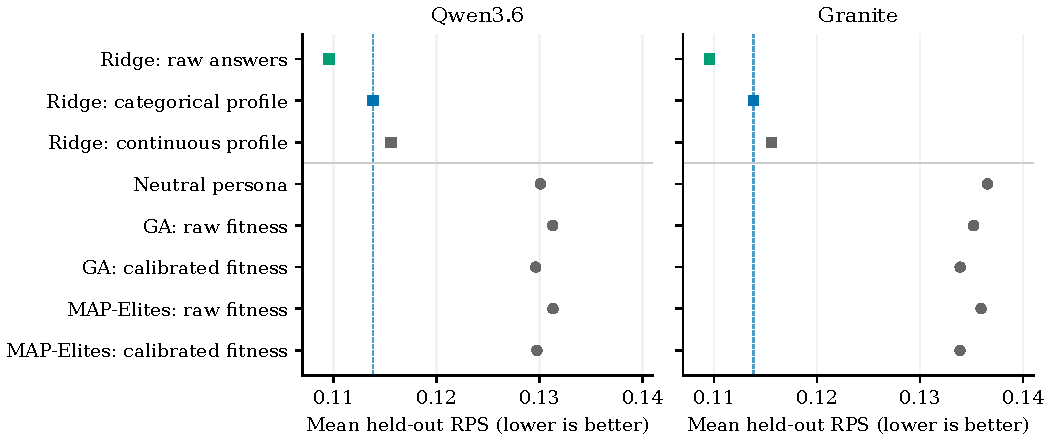
\includegraphics[width=.86\textwidth]{assets/492d193482a7.pdf}\end{center}
\noindent\textbf{Figure S3.} Full-data ridge and persona controls. Shared statistical predictors are repeated across panels for comparison. All ridge controls in this figure use 8,000 person-level labelled mappings. LLM arms use their frozen population calibration; ridge directly predicts ordinal CDFs. These are held-out RPS values, not an equal-supervision comparison. The dashed vertical line marks categorical-profile ridge.

\section{Associative label-budget diagnostics}
Two additional 48-test families cover the ordinary and shared-prior budget diagnostics, separately from the earlier 33 representation and nine objective contrasts.

The original 600-person cohort was already exposed. The ordinary-ridge diagnostic
was followed by a separate rival test using the 8,000-person empirical item prior.
Both are post hoc. For each fitting subset, the anchored variant predicts
\begin{equation}
\widehat F_{\rm anchored}(x)=\operatorname{Proj}\bigl(\widehat F_{\rm ridge}(x)+F_{0,8000}-\overline Y_{\rm subset}\bigr),
\end{equation}
where $\widehat F_{\rm ridge}$ is the unprojected intercept-fit ridge output and
$\overline Y_{\rm subset}$ the mean target-threshold vector. This changes only the
intercept at a given penalty; each variant selects its penalty on the same 120
selection people. It is algebraically centered no-intercept ridge about the
population prior. Using the original solver precision makes the full 8,000-point
correction zero and exactly reproduces every original individual loss.

\begin{table}[H]\centering\small
\caption{Mean RPS at each ridge fitting budget. Lower is better.}\label{tab:budget}
\begin{tabular}{@{}llrr@{}}\toprule
Features & Fit people & Ordinary & Shared prior\\\midrule
categorical & 80 & 0.13956 & 0.13802\\
categorical & 200 & 0.13150 & 0.13099\\
categorical & 320 & 0.12791 & 0.12759\\
categorical & 1,000 & 0.12069 & 0.12059\\
categorical & 8,000 & 0.11384 & 0.11384\\
categorical & exact 80 & 0.13814 & 0.13669\\
raw & 80 & 0.13795 & 0.13643\\
raw & 200 & 0.12972 & 0.12921\\
raw & 320 & 0.12607 & 0.12575\\
raw & 1,000 & 0.11824 & 0.11815\\
raw & 8,000 & 0.10955 & 0.10955\\
raw & exact 80 & 0.13624 & 0.13494\\
\bottomrule\end{tabular}\end{table}

Positive contrast values in the accompanying diagnostic files mean LLM minus
ridge RPS; negative values favour the LLM. Every variant has 48 comparisons:
2 representations times 6 fitting conditions times 4 GA model/objective arms.
Each family is separately Holm corrected. This does not correct for adaptively
choosing the second diagnostic after seeing the first. The full 48-row tables,
all subset means and frozen selection specifications are retained in the local
research artifact; no public data-release claim is made.

The ten fitting subsets per budget overlap. Their mean losses average separate
predictors, not ensemble probabilities; their min/max spread is not a confidence
interval. Crossed intervals resample only respondents and LLM search seeds,
conditioning on statistical fits and the population prior. Fitting counts omit
120 selection people. LLMs additionally use 120 calibration people and foundation-model
pretraining, so matching the empirical prior does not imply identical total
supervision or prove a causal sample-efficiency advantage. The exact 80 row uses
the original search people instead of training-panel subsets.

\section{Fitting-budget visualization}
\begin{center}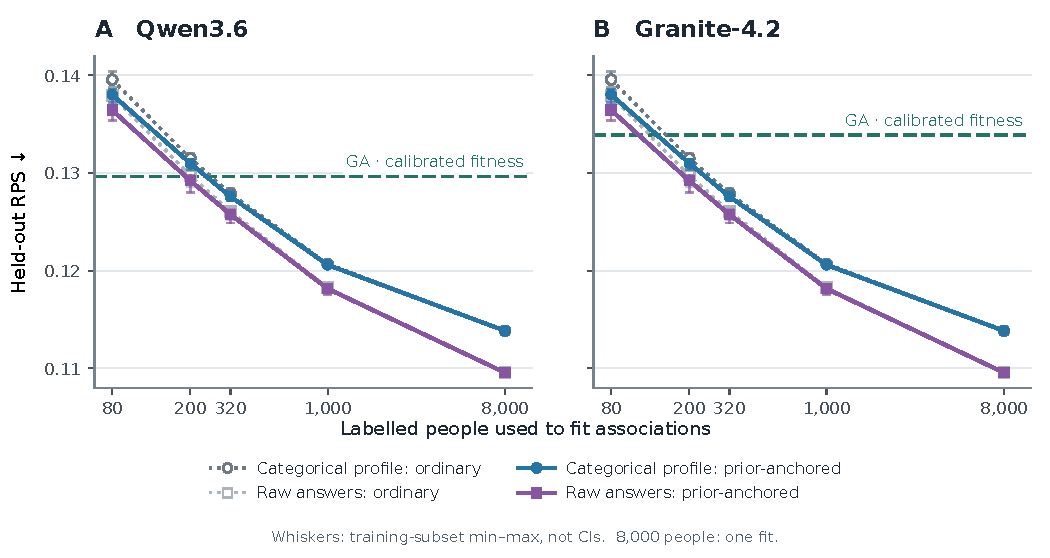
\includegraphics[width=.95\textwidth]{assets/8fc919841dd2.pdf}\end{center}
\noindent\textbf{Figure S4.} Ordinary and shared-prior ridge learning curves.
Whiskers are ranges across ten overlapping fitted subsets, not confidence
intervals. At 8,000 there is one fit. LLM lines average three frozen runs;
statistical curves repeat across model panels for comparison.

\section{Exploratory complementarity protocol}
We apply the established linear forecast pool~\cite{gneiting2011combining}:
\begin{equation}H_{ij}=(1-w)R_{ij}+wP_{ij},\qquad w\in\{0,.05,\ldots,1\}.\end{equation}
The convex combination is a valid CDF because both components are valid CDFs.
Ridge uses categorical or raw-answer features and nested subsets of 80, 200 or
320 training people, defined by seeds 202610081--202610083. It selects its
penalty on Select120. The first 60 ordered Calibrate people fit each persona's
scale and mean CDF; the last 60 choose the mixture weight. Neither calibration
nor mixture weights are refitted after selection. All three calibrated-GA runs
and their own neutral counterparts are retained. No new LLM calls are made.

The empirical prior uses Train8000 and the original prompt search uses
Search80/Select120. Each mixture requires the same last60 selection labels;
neutral and population mixtures independently select their weights. Thus all
supervision roles remain explicit. Train subsets overlap Train8000 and do not
represent additional distinct people. RPS first averages 60 items per person,
then averages losses over nine fixed fit/run combinations. This is not an
ensemble of nine prediction vectors. A single 48-test Holm family covers all
12 conditions against four controls. Intervals and sign flips use 5,000 paired
respondent draws with seed 20261008, conditional on these fixed fits. A useful
screen result requires gain at least 0.001, a positive 95\% interval and
Holm $p<.05$. All comparisons and nulls are retained. Selection parameters
were saved before explicit evaluation extraction; the full corpus and
evaluation-bearing result containers had already been loaded. This is a
procedural dataflow guard, not capability-level isolation; original full120-calibrated losses
reproduce exactly in all 12 base/evolved checks.



\clearpage
\setcounter{figure}{4}
\section{Complete complementarity results}
\begin{figure}[H]\centering
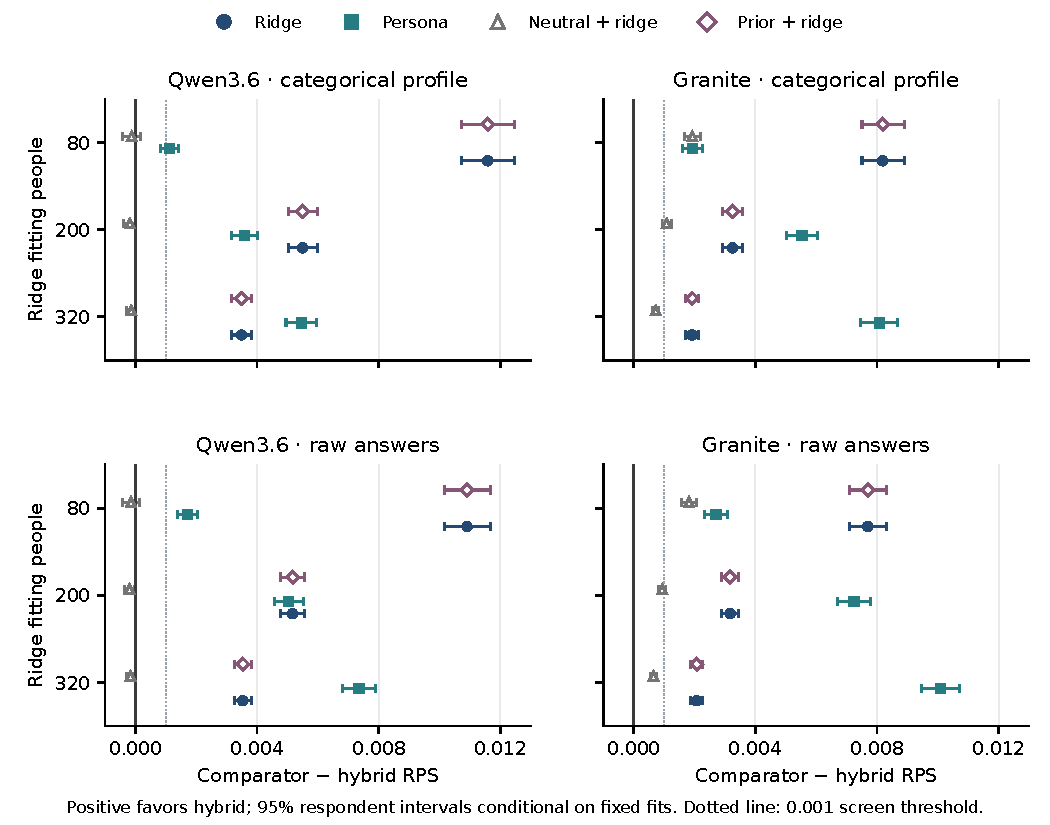
\includegraphics[width=.96\textwidth]{assets/38626aff3166.pdf}
\Description{All forty-eight mean score contrasts and respondent intervals across two models, two feature representations and three fitting budgets.}
\caption{All 48 contrasts: control minus optimized-persona mixture RPS.
Positive favors the mixture. Bars are respondent-bootstrap 95\% intervals
conditional on the fixed nine fits; the dotted line is the 0.001 screening
threshold. Color and marker identify the comparator. Full numerical means,
intervals and within-family Holm values are retained in the associated table.}
\end{figure}
Mixtures beat both standalone components in every condition. Optimization
itself passes the additional magnitude/statistical gate over the neutral
mixture only on Granite for categorical 80/200 and raw 80. No Qwen condition
passes that gate. The selected prior-mixture weights are all zero. Prior
mixing is a different comparator from refitting the intercept around the
population prior; the latter is tested separately below.
The analysis is adaptive on exposed respondents and complements, rather than
supersedes, earlier corpus-specific null evidence on persona combinations.

\clearpage
\section{Adversarial prior-anchored comparison}
After viewing the original screen, a separate protocol froze all 12 conditions
and the original hybrid forecasts. The two new rivals are the prior-anchored
ridge defined above, selecting its penalty on Select120, and a neutral-persona
mixture using that ridge. Neutral calibration uses the first 60 Calibrate
people and its independently selected mixture weight uses the last 60.
All 18 anchored fits reproduce the corresponding earlier individual losses
within $8.4\times10^{-17}$; original hybrid means are unchanged exactly.
No new LLM calls or GPU inference are used. The procedural evaluation guard
does not restrict the process's underlying file access.

The 24 contrasts form a separate Holm family with 5,000 paired respondent
bootstrap/sign-flip draws, conditional on the same nine fixed combinations.
The unchanged screening rule requires gain at least 0.001, positive marginal
95\% interval and adjusted $p<.05$. All twelve hybrids beat anchored ridge
by 0.00161--0.00984 RPS (all $p_{\rm H}=.0048$). Against neutral-plus-anchored
ridge, Granite gains 0.00044--0.00164; only categorical 80 and raw 80 also
clear the magnitude threshold. Qwen loses 0.00025--0.00038 in all six
conditions; five differences have $p_{\rm H}<.05$ and categorical 80 has
$p_{\rm H}=.0514$. Thus the stronger rival preserves the component-combination
result while narrowing the case for optimized personas. This remains adaptive
exposed-cohort evidence. Changing both the prompt and decoder makes the rival
a practical comparison, not a causal ablation of optimization.

\begin{figure}[H]\centering
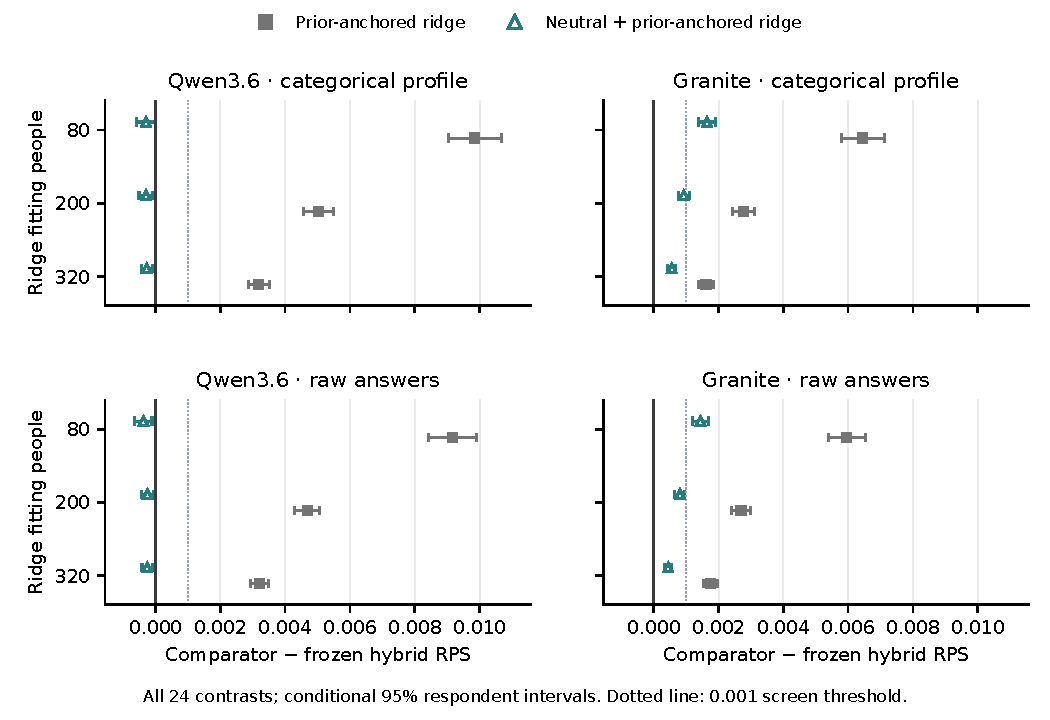
\includegraphics[width=.92\textwidth]{assets/426770f79060.pdf}
\Description{All twenty-four contrasts against stronger anchored ridge and neutral-plus-anchored controls, including negative Qwen differences.}
\caption{All 24 adversarial contrasts: comparator minus the unchanged original
hybrid. Bars are conditional respondent-bootstrap 95\% intervals; positive
favors the hybrid. The dotted line is the 0.001 screening threshold. All
conditions and unfavorable outcomes are retained; this family is separate
from the original 48 contrasts.}
\end{figure}

\clearpage
% Reproducibility appendix extracted on 2026-10-08 from the deployed source,
% immutable campaign manifest, and frozen result receipts. This is an \input{}
% fragment; it deliberately contains no respondent identifiers.
\section{Reproducibility specification}
\label{app:reproducibility}

\paragraph{Common execution contract.}
Every cell used the same Qwen/Qwen3.8-27B mutator, a strict mutable JSON genome,
temperature $0.7$, at most 2,500 generated tokens per ordinary mutation,
disabled thinking, and a fresh seeded mutator request.  The serialized genome has
exactly four top-level fields: \texttt{role\_definition}, fixed-length arrays of five
\texttt{trait\_formulations} and 30 \texttt{facet\_formulations}, and
\texttt{critic\_formulations}.  The runtime genotype also carries fixed
intensity modifiers copied from the neutral template; they are never mutated.
Malformed proposals consumed no forecast budget, whereas any mutator transport
failure invalidated the cell.  Search was capped at $B=80$ full optimization-panel
equivalents. Since the panel has 80 respondents and 60 target items, the cap
is $80\times80\times60=384{,}000$ respondent--item forecasts per cell;
realized search usage ranges from 78.2 to 80.0 equivalents.  The
separate shortlist stage rescored at most five candidates on 120 respondents
($7{,}200$ forecasts per candidate; at most $36{,}000$).  It selected the
lowest raw RPS with the genotype hash as a deterministic tie break.  Thus the
\texttt{generations}, \texttt{rounds}, and \texttt{iterations} fields below
describe the planned schedule; the forecast ledger, rather than those fields,
was the operative stopping rule.

\begin{table}[H]
\caption{Exact initialization, update/history, and budget-relevant parameters
for the eleven search methods.  ``Seed'' is the neutral genotype specified
below; all fitness comparisons minimize the cell's declared optimization
objective.}
\label{tab:repro-search}
\centering
\small
\setlength{\tabcolsep}{3pt}
\begin{tabular}{p{0.105\textwidth}p{0.19\textwidth}p{0.45\textwidth}p{0.19\textwidth}}
\toprule
Method & Initialization & Update and retained history & Fixed parameters \\
\midrule
GA & Seed plus mutations to population 8. & Two elites; two independent
tournament-$3$ parents.  LLM crossover with probability .8 when parents differ;
a crossed child is mutated with probability .3 and a copied parent is always
mutated. & Population 8; elites 2; tournament 3; crossover .8; mutation .3;
configured 10 generations. \\

Differential evolution & Same seed-plus-mutations population as GA. & For each
member $x$, sample three distinct other members $a,b,c$; the LLM applies the
$a-b$ difference to $c$ and crosses the result with $x$; greedily replace $x$
only on improvement. & Population 8; configured 10 generations.  The recorded
crossover-rate field is .8, but the deployed loop does not use it as a
stochastic gate. \\

Prompt-\allowbreak Breeder & Seed, then seven mutations using successive members of a fixed
eight-instruction mutation-prompt pool. & One elite; tournament-$3$ parent;
each member carries its mutation instruction.  With probability .25 the LLM
rewrites that instruction (temperature .9, 200 tokens), then applies it to the
parent genotype. & Population 8; instruction pool 8; hypermutation .25;
configured 10 generations. \\

MAP-Elites style & Two islands, four initial evaluations per island; only the
first is the unchanged seed, all others are seed mutations. & Uniformly sample
an occupied archive cell; mutate using the last six lineage records
(operation, score, prompt length, predicted SD); replace a cell only on lower
score; migrate the island champion every 12 iterations. & $2$ islands;
$4\times4$ bins with length edges $[0,1500,2500,$ $4000,100000]$ and SD edges
$[0,.8,1,1.2,9]$; 4 initial points/island; history 6; configured 72 iterations. \\

Local GEPA & Evaluate seed on the full panel and initialize a respondent-wise
Pareto pool. & Select a Pareto member in proportion to its number of
respondent-wise wins; compare parent and reflected child on the same eight
respondents; give the reflector the ten worst target-item errors; run a full
evaluation only after a minibatch improvement.  Retain the Pareto front and
global best; spend remaining whole equivalents on best-candidate mutations. &
Minibatch 8; at most 12 Pareto candidates; 10 feedback items; configured 80
evaluations. \\

\bottomrule
\end{tabular}
\end{table}
\begin{table}[H]\centering\small
\caption{Search specifications, continued. The same executed-forecast budget applies.}
\setlength{\tabcolsep}{3pt}
\begin{tabular}{p{0.105\textwidth}p{0.19\textwidth}p{0.45\textwidth}p{0.19\textwidth}}
\toprule
Method & Initialization & Update and retained history & Fixed parameters \\
\midrule
Official GEPA & Seed candidate and optimization respondents indexed $0$--$79$.
& GEPA v0.1.4 Pareto selection with per-example metric $-\mathrm{RPS}_{raw}$;
reflection minibatches of 8; merge disabled; no metric cache.  The external
forecast ledger is authoritative and returns the last fully scored elite at
exhaustion. & Reflection minibatch 8; package v0.1.4. \\

Native GigaEvo & Exact neutral JSON written as the initial program. & Pinned
native guided pipeline; single island without distant parents; no memory;
fitness $1-\mathrm{RPS}$; external validator and forecast stopper. & Internal
v2.20.1 at commit \texttt{f72ab08c}; maximum 160 mutants; concurrency 1;
$8\times8$ behavior space over length $[0,16000]$ and predicted SD $[0,2]$. \\

OPRO & Evaluate seed. & Propose in blocks of 8 from up to the 12 best valid
scored genotypes, printed from worse to better within that retained set. & 8
proposals/round; history 12; configured 10 rounds. \\

ProTeGi & Evaluate seed and start a beam. & For every beam member, generate two
textual-gradient edits using the ten worst target-item errors; evaluate one
edit per gradient; retain the best four candidates. & Beam 4; 2 gradients per
candidate; 1 edit/gradient; configured 20 rounds. \\

Random search & Evaluate seed. & Draw $B-1$ independent mutations of the seed;
return the best full-panel candidate. & 80 evaluations. \\

Best-of-$B$ & Evaluate seed. & Draw $B-1$ independent seed mutations with the
initial-population generator at temperature 1.0; return the best full-panel
candidate. & 80 evaluations; mutation temperature 1.0. \\
\bottomrule
\end{tabular}
\end{table}

\paragraph{Neutral genotype and exact rendering.}
The neutral role is: ``You are a simulated respondent. Answer each statement
according to the supplied personality profile.''  For each of the five
canonical traits $t\in\{$neuroticism, extraversion, openness, agreeableness,
conscientiousness$\}$, its exact formulation is ``Tendency toward $t$.''  For
each canonical facet label $f$ in the item key, the exact formulation is
``Tendency toward $\operatorname{lowercase}(f)$.''  The critic is: ``Use only
the supplied profile. Interpret the response scale consistently.''  Scores use
boundaries $[0,20,40,60,80,100]$ with labels \emph{very little}, \emph{slightly},
\emph{moderately}, \emph{quite strongly}, and \emph{very strongly}; operational
intervals are $[0,20)$, $[20,40)$, $[40,60)$, $[60,80)$, and $[80,100]$ after
endpoint clipping.

For a genotype $(r,T,F,c)$, the exact system-prompt skeleton is
\texttt{r\textbackslash nYour profile:\textbackslash n}, followed first by one
line per trait and then one per facet:
\texttt{- This trait (NAME) describes you MODIFIER: DESCRIPTION} and
\texttt{- This facet (NAME) describes you MODIFIER: DESCRIPTION}.  It ends with
\texttt{\textbackslash n\textbackslash nInternal reflection guideline:\textbackslash n}
and $c$.  A facet score is
$100(\bar{x}-1)/4$ from its two observed items; a trait score is the mean of its
six facet scores.

\paragraph{Selected wording example.}
The frozen Qwen calibrated-GA seed-1 template changes the neutral
``Tendency toward extraversion.'' to ``The intensity with which you derive
energy from social interaction, assertiveness, and positive emotional
experiences.'' Its critic includes: ``Avoid converging on a central tendency;
instead, maximize the semantic variance between answers to accurately reflect
the specific magnitude indicated, ensuring that a 'very little' response is
distinctly different from a 'slightly' one in both tone and content, so that
your agreement or disagreement scales linearly with the provided intensity.''
These are exact excerpts from one selected template, showing the intervention
on profile interpretation. They neither characterize every optimized template
nor establish a causal mechanism. The complete genotype accompanies the
source notes.

\paragraph{Items, people, and partitions.}
Items are grouped by facet after sorting by item number.  The first two items
of each of 30 facets form the 60-item observed input; the remaining two form
the disjoint 60-item prediction target.  Eligible rows have all 120 item values
in $\{1,2,3,4,5\}$, unique case IDs, and no match to the inventoried historical
exposure set.  Rows are sorted by case ID, permuted with seed 20261004, and
sliced without overlap into train/optimization/selection/calibration/evaluation
panels of 8,000/80/120/120/600 people (8,920 reserved rows).  A subsequent inventory records 410,168 complete cases, of which 374,049
match the accumulated exclusion set and 36,119 remain eligible in that
inventory. These are inventory counts, not a claim of new untouched test
people; all-host exposure coverage is unproven. The local reproducibility
bundle does not include the raw corpus, a verified dataset license, or
validated demographic summaries.  Sex, age, and
country are loadable fields, but no demographic interpretation or distribution
is asserted here.

\paragraph{Frozen exemplar and cryptographic closure.}
The saved Qwen calibrated-GA seed-1 selection has raw selection RPS
$0.1692038488$, five shortlisted candidates, and canonical selected-record hash
\texttt{4131b9d1dc37cd4f}; its complete runtime genotype is transcribed in the
accompanying source notes.  A second located exemplar, Granite calibrated
MAP-Elites seed 1, has selected-record hash \texttt{09d79eb1c951f4f8}.
The canonical manifest hash is \texttt{9037e61283d70779}; panel hash
\texttt{786de40844429e19}; frozen-record file hash \texttt{155b512315b52679};
final 84-cell recomputation hash \texttt{7a3009c03446254d}; model-lock file hash
\texttt{342d9215e991e973}; item-key hash \texttt{2cd1483c7d3d539c}; and deployed
source-closure hash \texttt{e333de246887ab0c}.  Full 64-hex digests, model
revision pins, source anchors, and the exact exemplar appear in
\texttt{REPRO\_SOURCE\_NOTES.md}.

\paragraph{Statistical predictors and score translation.}
The 60 ordinal targets are encoded as 240 indicators $\mathbf{1}[y_j\leq k]$
for $k=1,\ldots,4$. Raw inputs use 300 one-hot indicators; categorical inputs
use 175. Ridge fits an intercept with the Cholesky solver, without scaling
these one-hot features. Select120 minimizes RPS over penalties
$\{1,10,100,1000\}$, with smaller penalties breaking ties. Continuous-profile
features alone are standardized using training statistics. Predictions undergo
the exact squared-error projection of each four-threshold vector onto
$0\leq F_1\leq\cdots\leq F_4\leq1$. ExtraTrees uses 64 trees,
minimum leaf size selected from $\{10,30\}$, feature fraction .8, random seed
20261004, one worker, and otherwise scikit-learn defaults. Answer-equivalent
curves use a nonincreasing isotonic fit and linear interpolation over the
registered budget grid; out-of-grid values remain censored. Their bootstrap
resamples respondents and the three fixed input orders, not training fits.

\paragraph{Pinned model revisions.}
The full model revision pins are:
\begin{quote}\small
Qwen predictor: \texttt{995ad96eacd98c81ed38be0c5b274b04031597b0}\\
Granite predictor: \texttt{9e668ce1c538387ef24d3644e9b0606647762636}\\
Qwen mutator: \texttt{1d4bf0f2ff6012fd82039f2fa52739d0dd7c60c0}.
\end{quote}
The documented analysis environment uses Python 3.12.14, NumPy 2.3.5,
scikit-learn 1.7.2, and serving vLLM 0.28.0. Full source notes and receipts
are retained locally; no publicly executable anonymous artifact is claimed.


\begin{table}[H]\centering\small
\caption{All exploratory mixture conditions: mean RPS, lower is better.
Each mean averages losses of the nine fixed fits. The preceding forest plot
shows every paired contrast and its conditional interval.}
\begin{tabular}{@{}llrrrrrr@{}}\toprule
Model & Features & Fit $n$ & Hybrid & Ridge & Persona & Neutral mix & Prior mix\\\midrule
Qwen & categorical & 80 & 0.12859 & 0.14017 & 0.12972 & 0.12846 & 0.14017\\
Qwen & categorical & 200 & 0.12613 & 0.13163 & 0.12972 & 0.12595 & 0.13163\\
Qwen & categorical & 320 & 0.12427 & 0.12776 & 0.12972 & 0.12413 & 0.12776\\
Qwen & raw & 80 & 0.12800 & 0.13891 & 0.12972 & 0.12786 & 0.13891\\
Qwen & raw & 200 & 0.12468 & 0.12984 & 0.12972 & 0.12448 & 0.12984\\
Qwen & raw & 320 & 0.12237 & 0.12590 & 0.12972 & 0.12221 & 0.12590\\
Granite & categorical & 80 & 0.13198 & 0.14017 & 0.13392 & 0.13392 & 0.14017\\
Granite & categorical & 200 & 0.12838 & 0.13163 & 0.13392 & 0.12946 & 0.13163\\
Granite & categorical & 320 & 0.12584 & 0.12776 & 0.13392 & 0.12656 & 0.12776\\
Granite & raw & 80 & 0.13121 & 0.13891 & 0.13392 & 0.13303 & 0.13891\\
Granite & raw & 200 & 0.12667 & 0.12984 & 0.13392 & 0.12761 & 0.12984\\
Granite & raw & 320 & 0.12383 & 0.12590 & 0.13392 & 0.12448 & 0.12590\\
\bottomrule\end{tabular}\end{table}

\section{AI-assistance record}
This revision additionally used Claude Code for independent manuscript critique and Codex for analysis, editing and plotting; the main paper states the combined disclosure. Historical records below concern earlier stages.

Codex assisted source inspection, experiment specification, coding and writing;
retained review records identify GPT-5.6-Sol for draft and claim review.
Retained Claude artifacts document generic figure-layout assistance; research
labels and numerical values were bound and checked locally. Available records
are inventoried in \texttt{AI\_CONTRIBUTION\_LEDGER\_20261020.json} in the
research evidence directory, including artifact hashes and coverage limits.
This is a partial record: complete prompt/response retention and independently
attested model identities are unavailable. Exact versions and prompts for older
unrecorded interactions remain unknown.

\section{Exploratory mixture uncertainty}
\begin{figure*}[t]
\centering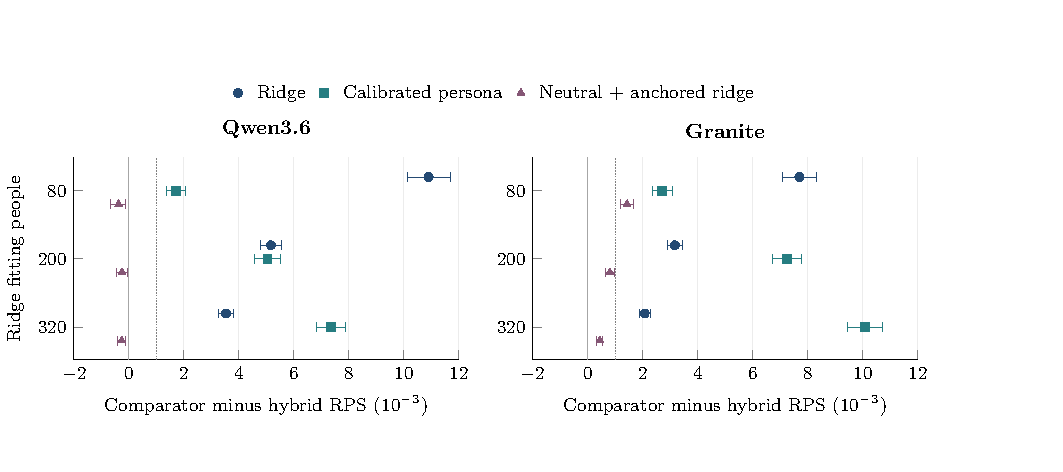
\includegraphics[trim={0 .75cm 1.5cm 1.2cm},clip,width=.96\textwidth]{assets/b5f29adb5aa2.pdf}
\Description{Two model panels show raw-answer hybrid gains over ridge,
calibrated persona, and the stronger neutral-plus-anchored-ridge rival at
three fitting budgets. Intervals are conditional on fixed fitted predictors;
the stronger neutral rival beats the hybrid in all three Qwen conditions.}
\caption{Exploratory paired gains on the exposed 600 respondents (raw-answer
features). Positive values favor the optimized-persona mixture; bars are 95\%
respondent intervals conditional on nine fixed fit/run combinations. The
vertical dotted line marks the 0.001 practical threshold. Component comparisons
belong to the 48-test family; the stronger neutral rival to the separately
frozen 24-test family. Intervals are pointwise. All LLMs also use the
8,000-person prior; small fitting counts are not total supervision budgets.
The supplement includes categorical features and every declared comparison.}
\label{fig:hybrid}
\end{figure*}

\section{Original-cohort objective effects}
\begin{figure*}[t]
\centering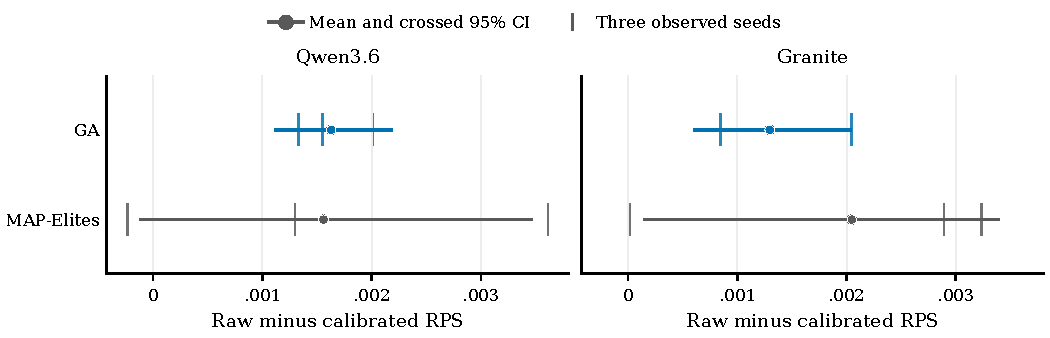
\includegraphics[width=.96\textwidth]{assets/9fc06813afc7.pdf}
\Description{Two model panels show three paired seed effects and pooled
crossed intervals for GA and MAP-Elites. Positive raw-minus-calibrated RPS
favors calibrated fitness. Qwen MAP-Elites includes a negative seed effect.}
\caption{Direct objective effects, post-hoc analysis. Ticks show
three paired seed effects; circles and bars show means and crossed
95\% intervals. Positive values favor calibrated fitness. All observed GA
seeds favor calibrated fitness, but three seeds do not establish generalization
over optimizer randomness. Original comparisons remain in
the main complete-comparison tables.}
\label{fig:objective}
\end{figure*}

\section{Detailed original-cohort budget and mixture diagnostics}
\subsection{Exploratory fitting-budget diagnostics}
On the exposed cohort, shared-prior statistical controls have higher mean RPS
than calibrated GA at 80 fitting people but lower mean RPS at 320; the
supplement reports full learning curves and supervision counts.

Using the exact 80 search respondents, common-prior categorical ridge scores
0.13669. Calibrated GA is lower by 0.00705 on Qwen and 0.00278 on Granite.
Against the stronger raw-answer control (0.13494), the Qwen difference is
$-0.00530$ (crossed interval $[-0.00638,-0.00422]$, conditional Holm
$p=.0096$); Granite's $-0.00103$ contrast does not satisfy the combined
decision rule ($p=.0656$). Thus a restricted positive Qwen result survives
the shared-prior check, whereas a cross-model claim against that control
does not. The LLM still uses 120 additional calibration people and pretrained
parameters; the ridge fitting count excludes its 120 selection people.
These diagnostics neither establish equal-total-budget efficiency nor select
an optimal budget on unexposed data.



Under the frozen ridge input curve, the primary Qwen persona corresponds
to 10.97 answers (conditional 95\% interval $[9.06,12.92]$) and Granite to
7.51 ($[6.36,8.84]$). These intervals propagate respondent and nested-order
variation after averaging the three persona seeds; they do not propagate
fresh optimizer-seed uncertainty. All 84 search curves reach 78.2--80
full-panel equivalents. Their checkpoints describe development efficiency,
not a second procedure for selecting on evaluation respondents.

\subsection{Exploratory complementarity}
The selected persona--ridge mixture improves over both components in all
12 conditions under the screen rule. Gains over ridge range from 0.00192 to
0.01158 RPS, and gains over the calibrated persona from 0.00113 to 0.01009
(all conditional Holm $p=.0096$). The supplement shows paired gains and uncertainty for both representations
and all 48 contrasts.
No new model inference was needed: the experiment reuses saved forecasts,
with calibration fitting and mixture selection separated.

The selected mixtures had lower RPS on this exposed cohort; the neutral
control separates this observation from optimizer value. On Granite, the optimized mixture has lower
mean RPS than the neutral mixture in all six conditions; three pass the
0.001 magnitude threshold as well as the statistical rule (categorical 80/200,
raw 80). On Qwen, all six neutral mixtures have slightly lower means, with no
significant difference after correction. Population-mixture selectors choose
zero prior weight throughout, reproducing ridge. This linear-pool control is
distinct from the earlier prior-anchored intercept refit. The observed advantage of combining predictors spans both tested models,
while additional utility from persona search remains model- and budget-specific.

A separately frozen adversarial extension tests prior-anchored ridge and
neutral-plus-anchored ridge in all 12 conditions (24-test Holm family).
The original hybrid beats anchored ridge throughout, by 0.00161--0.00984 RPS
(all $p_{\rm H}=.0048$). Against the stronger neutral mixture, only Granite
categorical/raw 80 clear the magnitude/statistical rule. Qwen loses in all
six conditions, five significantly. This practical rival changes both prompt
and decoder; it is not a pure optimizer ablation or independent confirmation.




\section{Detailed saved-forecast protocols}
After inspecting the original evaluation, we fixed the following saved-forecast
analyses before executing them. They reuse the exposed 600-person cohort and
are \emph{post hoc}, not independent confirmation. Within these diagnostics,
no prompts are changed and no new LLM predictions are generated. The original
110-test analysis is retained.

Representation controls compare the exact 175 one-hot profile features
visible in prompts with 35 continuous pre-discretization values and raw
history. All use Train8000 and Select120; original losses reproduce within
$10^{-10}$. Separate Holm families cover 33 representation contrasts and
nine objective/optimizer contrasts. Rank diagnostics retain the first
complete evaluation per genotype in all 24 GA/MAP search pools.

Budget diagnostics fit categorical and raw-history ridge at 80, 200, 320,
1,000 and 8,000 people and exact Search80. Ten fixed nested subsets per
smaller budget share Select120 penalty choice. A subsequent prior-anchored
control replaces the subset target mean with the Train8000 prior. Both
curves reproduce full-data losses. Each has a separate 48-test family;
intervals condition on fits and resample respondents and observed LLM runs.
Subset ranges are not confidence intervals. Full specifications and the
adaptive exposure history are in the supplement.

\paragraph{Exploratory forecast combination.}
A final fixed screen tests complementarity using a linear pool of ordinal
CDFs~\cite{gneiting2011combining}, $H=(1-w)R+wP$, where $R$ is ridge and $P$
a calibrated-GA persona. Both models, both ridge representations and fitting
sizes 80, 200 and 320 are included. Three fixed nested training subsets cross
all three saved optimizer runs. Ridge penalties use Select. The first 60
Calibrate people fit the persona scale and center; the remaining 60 select
$w\in\{0,.05,\ldots,1\}$ by RPS. Parameters are fixed before evaluation.
Controls are ridge, persona, neutral-persona plus ridge, and population-prior
plus ridge; each mixture tunes its own weight on the same 60 people.
A separate 48-test Holm family and 5,000 respondent-bootstrap draws condition
on the nine fixed fit/run combinations. The screen requires mean gain at least
0.001, a positive gain interval and adjusted $p<.05$. All 12 conditions are
reported. This adaptive analysis reuses the exposed cohort and the 8,000-person
prior; low ridge fitting counts do not mean low total supervision.


\section{Detailed representation contrasts}
The additional categorical-profile ridge scores 0.11384, compared with
0.11558 for continuous-profile ridge and 0.10955 for raw-history ridge
(Supplementary Figure S3). Its deficit to raw-history ridge is
0.00428 (paired respondent interval $[0.00378,0.00478]$), while every LLM
arm is 0.01581--0.02388 worse than categorical ridge; all 28 intervals are
positive with Holm $p<.01$ in the 33-test family. Neutral personas also lose
by 0.01625 on Qwen and 0.02273 on Granite. The profile retains information
usable by a simple predictor even when persona search adds little. Ridge fits
8,000 person-level labelled mappings; the LLM pipeline uses those labels for
item priors, while prompt optimization uses 80 search and 120 selection people.
Thus person-level supervision budgets are not matched. This does
not equate their learning procedures or give a causal compression/readout
decomposition.

Relative to the empirical prior, categorical ridge retains
$(0.15174-0.11384)/(0.15174-0.10955)=89.8\%$ of raw-history ridge's
RPS improvement. This is an observed prediction-improvement ratio, not a
fraction of human information. Calibrated GA and MAP-Elites recover only
2.1\% and 1.6\% of their base-to-raw-ridge gaps on Qwen and 9.8\% and
9.9\% on Granite. These descriptive ratios have no additional significance claim.



\bibliographystyle{plainnat}\bibliography{references}\end{document}